\subsection{Grundkonzept}

Das zentrale Alleinstellungsmerkmal von \coc\ ist der neu entwickelte Gameplay Loop innerhalb der einzelnen Level. 
Die Encounter-Karten (siehe \Cref{fig:e_card_example}) liegen in einer Reihe vor dem Spieler und müssen nacheinander oder in einer strategisch sinnvollen Reihenfolge gespielt werden. 
Jede Karte besitzt Kosten in den drei Ressourcen Feuer, Wasser und Natur, die zum Spielen der Karte ausgegeben werden müssen.
Die Besonderheit besteht darin, dass die Summe der reinen Kartenkosten bewusst höher ist als die Ressourcen, die dem Spieler unmittelbar zur Verfügung stehen. 
Ein Level lässt sich daher nicht lösen, indem einfach jede Karte der Reihe nach bezahlt wird. 
Stattdessen muss der Spieler die Effekte, Bedingungen und individuellen Mechaniken der Karten gezielt nutzen, um mit seinen begrenzten Ressourcen das Level zu lösen.
Einige Karten geben beispielsweise beim Bezahlen neue Ressourcen. 
Andere reduzieren die Kosten benachbarter Karten um bestimmte Ressourcenarten. 
Viele Effekte sind zudem an Bedingungen geknüpft: Manche Karten entfalten ihre Wirkung nur, wenn sie zwischen Karten einer bestimmten Farbe liegen, andere müssen neben einer gleichartigen Karte oder am Rand der Kartenreihe positioniert werden, damit sich ihre Effekte gegenseitig aktivieren.
Zusätzlich existieren zeitabhängige Mechaniken, bei denen sich Karten beispielsweise in einem periodischen Rhythmus verändern und etwa während jeder dritten Spieleraktion günstiger werden.
Dadurch entsteht bereits auf Ebene der Encounter-Karten ein vielschichtiges Puzzle. 
Der Spieler muss gleichzeitig berücksichtigen, in welcher Reihenfolge er die Karten bezahlt, welche Ressourcen dadurch entstehen oder eingespart werden, wie die Karten zueinander positioniert sind und zu welchem Zeitpunkt bestimmte Aktionen ausgeführt werden.

\begin{figure}
    \centering
    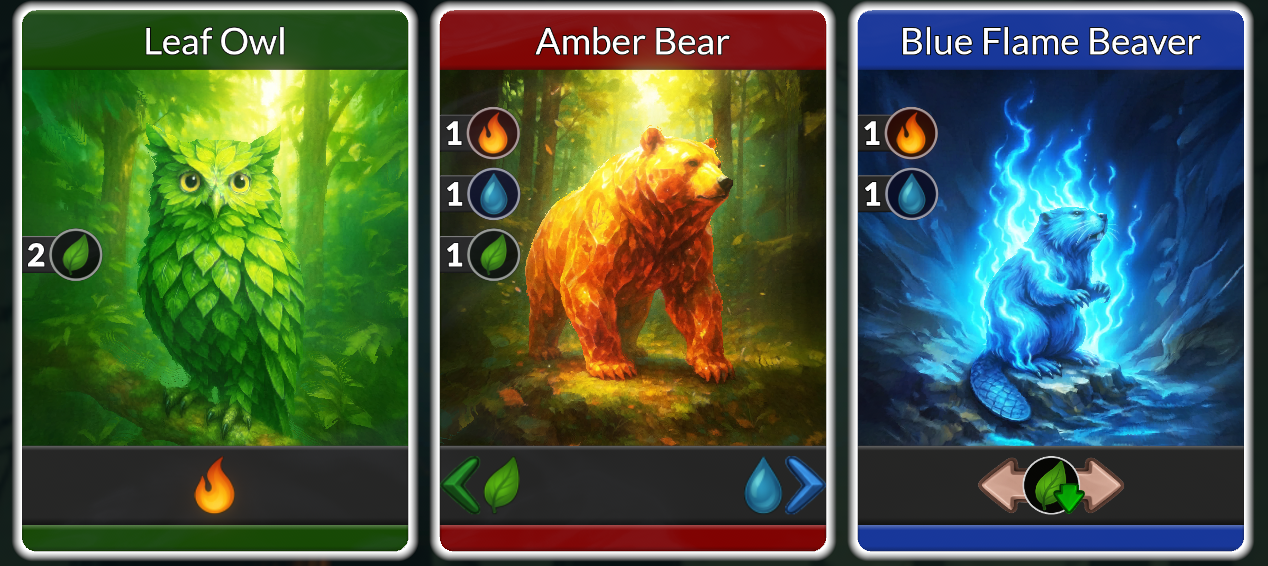
\includegraphics[width=1\linewidth]{img/CoC_e_cards_example.png}
    \caption{Encounter-Karten. Encounter-Karten können grün, rot oder blau sein, eine oder mehrere der Ressourcen Feuer, Wasser und Natur kosten (jeweils links) sowie unterschiedliche Effekte oder Bedingungen haben (jeweils unten).}
    \label{fig:e_card_example}
\end{figure}

\subsubsection{Zauberkarten und Bewegungsfähigkeiten}
Um die Level zu lösen, stehen dem Spieler zusätzlich Zauberkarten zur Verfügung.
Zauber erweitern das durch die Encounter-Karten entstehende Puzzle um eine weitere Ebene, indem sie dem Spieler erlauben, die bestehende Situation gezielt zu beeinflussen.
Ein wichtiger Teil dieser Fähigkeiten verändert die Position der Encounter-Karten, da diese in \coc\ eine zentrale strategische Rolle spielt. 
Unterschiedliche Zauber verfolgen dabei bewusst unterschiedliche Ansätze. 
Beispielweise gibt es Zauberkarten, die zwei benachbarte Karten tauschen oder eine Karte über mehrere andere hinweg verschieben.
Andere Zauber ermöglichen es, einzelne Karten für eine bestimmte Anzahl von Aktionen vollständig aus der Reihe zu entfernen oder eine Karte hinter einen anderen zu \glqq verstecken\grqq, sodass erst das Bezahlen der vorderen Karte die hintere wieder ins Spiel bringt.
Dadurch können Bedingungen auf Encounter-Karten gezielt hergestellt, aufgelöst oder zu einem günstigeren Zeitpunkt aktiviert werden.
Andere Zauber greifen an völlig anderen Stellen in das System ein: Sie können Kartenkosten reduzieren, zusätzliche Ressourcen erzeugen, Karten verwandeln oder duplizieren, Statuseffekte anwenden oder auf bestimmte Karteneigenschaften und bereits vorhandene Synergien reagieren. 
Unterschiedliche Zauber eröffnen dadurch unterschiedliche Lösungswege für dieselbe Spielsituation.
Der eigentliche spielerische Anspruch entsteht somit aus dem Zusammenspiel mehrerer Ebenen: Ressourcenmanagement, Aktionsreihenfolge, Positionierung, Timing, Kartenmechaniken und der strategische Einsatz der eigenen Zauber. 
Ein Level ist dadurch weniger mit einem klassischen Kartenkampf vergleichbar als mit einer dynamischen und strategischen Problemstellung, deren Ausgangszustand durch gezielte Manipulation in eine lösbare Situation überführt werden muss.

\subsubsection{Unterschiede zu Deckbuilding-Spielen}
Der zentrale Gameplay Loop von \coc\ unterscheidet sich von klassischen Deckbuilding-Kartenspielen insbesondere durch den hohen Stellenwert von Vorausplanung, Reihenfolge und Zustandsveränderungen innerhalb eines Levels.
In vielen Deck-building-Spielen besteht ein wesentlicher Teil der Spielerfahrung darin, die aktuell gezogene Kartenhand möglichst effizient zu nutzen.
Nachdem diese ausgespielt wurde, entsteht mit der nächsten Hand eine neue Situation, auf die der Spieler erneut reagieren muss.
Strategische Planung findet zwar statt, wird jedoch fortlaufend durch das Ziehen neuer Karten und damit durch neue, zuvor nicht vollständig bekannte Handlungsmöglichkeiten geprägt.
In \coc\ liegt dagegen ein großer Teil der relevanten Information bereits offen vor dem Spieler. 
Die Encounter-Karten, ihre Kosten, ihre Effekte, ihre Positionen sowie die eigenen verfügbaren Zauber sind bekannt. Dadurch können nicht nur einzelne Aktionen optimiert, sondern ganze Aktionsfolgen im Voraus geplant werden.
Dabei verändert nahezu jede Entscheidung die nachfolgende Spielsituation. 
Wird eine Encounter-Karte bezahlt und aus der Reihe entfernt, rücken die verbleibenden Karten zusammen und bilden neue Nachbarschaften. 
Dadurch können Bedingungen anderer Karten plötzlich erfüllt oder aufgehoben werden. 
Gleichzeitig werden Ressourcen ausgegeben oder durch Karteneffekte zurückgewonnen, Kosten anderer Karten verändert und zeitabhängige Mechaniken um eine weitere Aktion vorangetrieben. 
Auch der Einsatz von Zaubern kann Positionen, Kartenarten, Kosten oder andere Eigenschaften verändern und damit wiederum spätere Aktionen vorbereiten.
Der Spieler muss daher nicht nur entscheiden, welche Aktion aktuell vorteilhaft ist, sondern welche Reihenfolge von Aktionen das Level insgesamt in einen lösbaren Zustand überführt. 
Eine zunächst ungünstige Aktion kann beispielsweise notwendig sein, um Karten zusammenrücken zu lassen, dadurch einen Effekt zu aktivieren, neue Ressourcen zu erhalten und erst mehrere Schritte später eine besonders teure Karte bezahlen zu können.
Der Gameplay Loop ähnelt damit stärker einem strategischen, dynamischen Puzzle mit weitgehend vollständiger Information als einer fortlaufenden Optimierung zufällig entstehender Kartenhände. 
Die Herausforderung entsteht aus dem Zusammenspiel von Ressourcenmanagement, Aktionsreihenfolge, Positionierung, Timing, Kartenmechaniken und Zaubern und ermöglicht dadurch eine wesentlich stärkere Vorausplanung über mehrere miteinander verknüpfte Spielzüge hinweg.

\subsubsection{Zugänglichkeit und Lernkurve}
Trotz seiner strategischen Tiefe soll \coc\ einen sehr zugänglichen Einstieg bieten. 
Das grundlegende Ziel eines Levels ist unmittelbar verständlich: Karten besitzen Kosten in wenigen, klar unterscheidbaren Ressourcen und müssen durch den gezielten Einsatz dieser Ressourcen und der verfügbaren Fähigkeiten aufgelöst werden.
Die Komplexität entsteht erst schrittweise durch zusätzliche Karteneffekte, Bedingungen, Positionierungsregeln, Timing-Mechaniken, Zauber und weitere Systeme. 
Neue Elemente können dadurch auf einem bereits verstandenen Fundament aufbauen, anstatt den Spieler zu Beginn mit der gesamten Systemtiefe gleichzeitig zu konfrontieren.
So soll eine Lernkurve entstehen, bei der der zentrale Gameplay Loop schnell verständlich und spielbar ist, das Spiel jedoch mit zunehmender Erfahrung kontinuierlich neue Zusammenhänge, Interaktionen und strategische Möglichkeiten eröffnet. 
Die langfristige Tiefe entsteht damit nicht aus einem komplizierten Einstieg, sondern aus der schrittweisen Kombination zunächst leicht verständlicher Einzelmechaniken.

\subsubsection{Spielmodi}
Der puzzle-artige Core Gameplay Loop von \coc\ bildet die Grundlage von zwei verschiedenen Spielmodi, dem \textbf{Challenge-Modus} und dem \textbf{Roguelite-Modus}. 
Beide verwenden dieselben grundlegenden Mechaniken, stellen jedoch bewusst unterschiedliche Anforderungen an den Spieler, die auf deutlich unterschiedliche Spielerfahrungen abzielen.

Im \textbf{Challenge-Modus} geht es darum, jeweils alleinstehende, handgefertigte Level (`Challenges') zu verstehen und zu lösen.
Jedes Level bildet eine eigenständige strategische Problemstellung und kann beliebig oft wiederholt werden. 
Der Spieler kann unterschiedliche Ansätze ausprobieren, Zusammenhänge verstehen und so lange experimentieren, bis er eine Lösung findet.
Die Level werden dabei nicht lediglich zunehmend schwieriger, sondern stellen den Spieler immer wieder vor qualitativ neue Fragestellungen und Kombinationen bereits bekannter Mechaniken.
Damit ein besonders schwieriges Level den Spielfortschritt nicht blockiert, können Challenges übersprungen und später erneut gespielt werden. 
Auf Wunsch kann zudem eine Lösung angezeigt werden. 
So können die Puzzle anspruchsvoll bleiben, ohne vorauszusetzen, dass jeder Spieler jede Aufgabe selbstständig lösen muss.

Im \textbf{Roguelite-Modus} werden mehrere Level zu einer zusammenhängenden Reise verbunden, mit dem Ziel, dass der Spieler seine Strategie kontinuierlich weiterentwickelt, seine Zauberfähigkeiten verbessert und sich so zunehmend herausfordernden Levels stellen kann.
Der Roguelite-Modus bildet das Herzstück von \coc\ und wird im folgenden Abschnitt genauer detailliert.

\subsubsection{Level Editor}
Zusätzlich zum Spielen im Roguelite-Modus oder dem Lösen vorgefertigter Challenges soll es auch einen Level-Editor geben, der es Spielern ermöglicht, auf Grundlage der vorhandenen Karten, Zauber und Spielmechaniken eigene Level zu erstellen und anschließend mit anderen Spielern zu teilen.
Für die Erstellung eines Levels können die verfügbaren Encounter- und Zauber-Karten nach Name, Effekten und Kosten gefiltert und gezielt hinzugefügt, umsortiert oder entfernt werden. 
Für jeden einzelnen Zauber kann zudem festgelegt werden, welche Upgrades aktiviert sind. 
% Über Upgrades ist streng genommen hier noch nicht geredet worden.
Dadurch können sowohl einfache Puzzle mit wenigen Mechaniken als auch gezielt auf bestimmte Fähigkeiten, Synergien oder komplexe Interaktionen zugeschnittene Challenges konstruiert werden.
Ein erstelltes Level kann jederzeit direkt im Editor getestet werden. 
Gelingt es dem Ersteller, das Level während eines solchen Tests erfolgreich zu lösen, wird die dabei verwendete Lösung gespeichert und das Level als \glqq lösbar\grqq\ gekennzeichnet. Wird das Level anschließend verändert, beispielsweise durch das Austauschen einer Karte, eine veränderte Reihenfolge oder eine andere Zauberauswahl, so verliert es diese Markierung automatisch und muss erneut erfolgreich getestet werden.
Nur als lösbar verifizierte Level können veröffentlicht und mit der Community geteilt werden. 
Dadurch wird sichergestellt, dass veröffentlichte Challenges zumindest nachweislich eine funktionierende Lösung besitzen, ohne den Spielern vorzugeben, dass dies die einzige oder optimale Lösung sein muss.
Andere Spieler können veröffentlichte Level anschließend herunterladen, spielen und bewerten. 
Auf diese Weise soll langfristig neben den von uns entwickelten Challenges ein zusätzlicher Pool an nutzergenerierten Inhalten entstehen. 
Besonders interessante, kreative oder anspruchsvolle Kombinationen der vorhandenen Mechaniken können so von der Community selbst entdeckt und weitergegeben werden.
Eine frühe Version dieses Editors ist bereits Bestandteil unseres aktuellen Entwicklungsstands und wird intern zur Erstellung eigener Level genutzt. 
Die grundlegende Funktionalität zur Zusammenstellung und Anpassung von Levels ist damit bereits erprobt. 
Im Rahmen der weiteren Entwicklung soll dieses interne Werkzeug zu einem zugänglichen Community-Editor ausgebaut und um Funktionen zum Validieren, Veröffentlichen, Teilen und Bewertung ergänzt werden.
Der Editor erweitert damit nicht nur den Umfang des Spiels, sondern nutzt zugleich die puzzle-artige Struktur des zentralen Gameplay Loops, um langfristig neue Inhalte über die eigentliche Entwicklungsphase hinaus entstehen zu lassen.
